\section{Event Module}
\subsection{Overview}
The Event module is responsible for the Event Management for example lectures, Programs, tests and events.
 
\subsection{External Interface Requirements}
This section gives a detailed description of the system interfaces, hardware interfaces, software interfaces as well as communication interfaces. 

	\subsubsection{System Interfaces}
		\begin{itemize}
			\item The user module will interface with any subsystem or module that wants to access Events.

			\item  The user module will interface with Notification to Notify User about Events
		
		\end{itemize}
	\subsubsection{User Interfaces }
	\begin{itemize} 

	\item User Interface is in Calander Form which Shows all the events in it.

 \end{itemize}
 
	\subsubsection{Hardware Interfaces }
	The Event Module does not have any explicit hardware interface

	\subsubsection{Software Interfaces } 
	The event module will communicate with the database in order to get the details of events, and also for saving and editing new Events etc. All the I/O interaction with the database.
	
	\subsubsection{Communication Interfaces } 
		\begin{itemize}
		\item The Event module will need to comunicate with Notification to notify Users.
		\item needs to comunicate with Users as only registered user can see Events.
		\end{itemize}

	
\subsection{Performance Requirements}
Event module should be able to perform under high CRUD operations,and have optimised methods to allow for faster execution and faster response times.


\subsection{Design Constraints}
\begin{itemize}

\item The speed at which NavUP can perform is constrained by the processing power and the  memory that is available on the device on which it runs.

\item This system’s ability to give updates and events to users through the Users module is constrained by the external management and maintenance which is performed by the administrator of the system.

\end{itemize}


\subsection{Software System Attributes} 
\subsubsection{Availability}
The Event module should always be active since the it has Time Countdown and also there is posibility od Changing and updating all the time. 
\subsubsection{Reliability}
The Event module should make use of queuing for CRUD database operations, which most databases have and should be reliable since the database should be ACID compliant.

\subsubsection{Security}
Data within the Event module should not have external classes accessing the information without being authenticated, only admins can modify Events and add them or remove it, so No Guest or Normal User must be able to access to editing functionalities, also not registered User cannot see Events.

\subsubsection{Auditability}
As Admin,Normal and Guest Users have different Authorities to View and Modify Events, so user must be Logged on the Back-end Server before Getting to Events section

 
\subsection{UML}
\subsubsection{Class Diagram}
The class diagram of the Events sub-system makes use of the template method design pattern so that if need be one can easily construct different types of Event with minimal code modifications.

\begin{figure}[H]
	\centering
	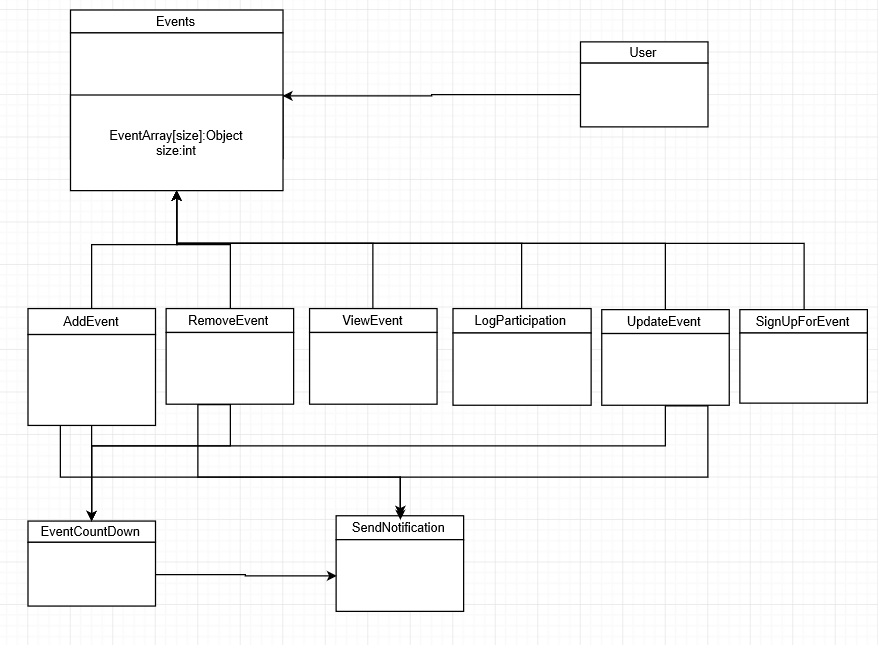
\includegraphics[width=0.7\textwidth]{event/ClassDiagrams(NoMethods).PNG}
	\caption{Event Class Diagram}
\end{figure}



\pagebreak
\subsubsection{Activity Diagram}
This diagram models work-flow activities of what users can do in the Event module.

\begin{figure}[H]
		\centering
		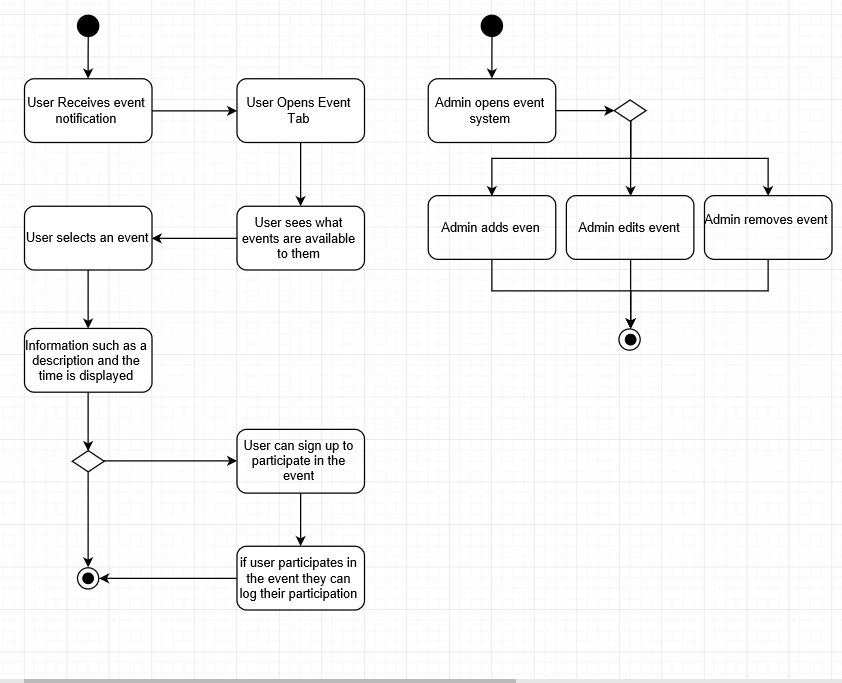
\includegraphics[width=\textwidth]{event/ActivityDiagramTask2.PNG}
		\caption{Events Activity Diagram}
\end{figure}


\subsubsection{Sequence Diagram}
This diagram models time-ordered interaction behaviour between a user logging in and the interaction with the Event subsystem.
\begin{figure}[H]
		\centering
		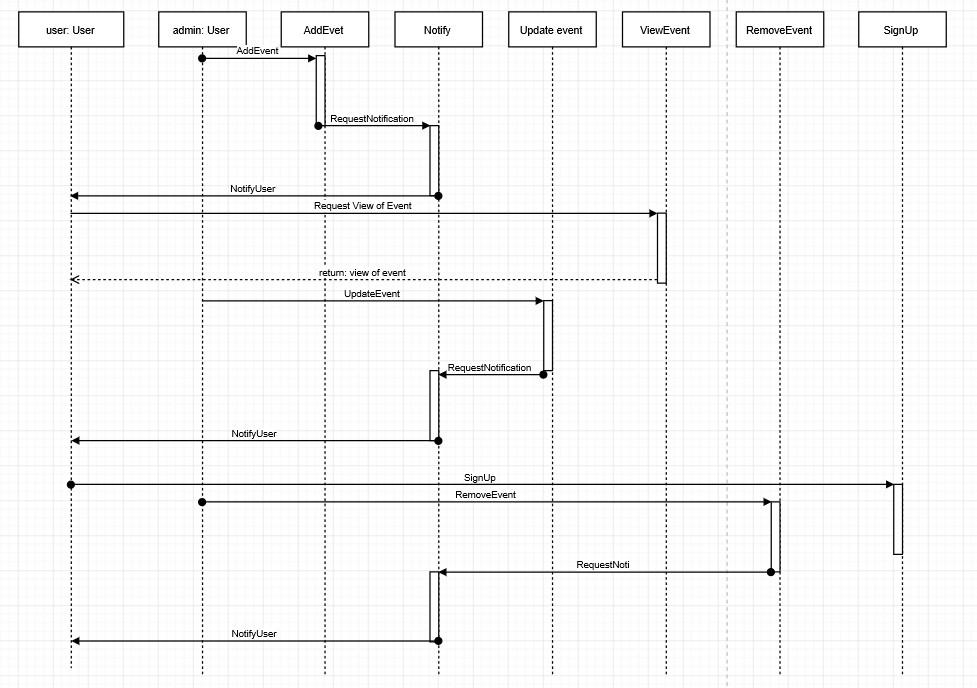
\includegraphics[width=0.7\textwidth]{event/SequenceDiagramTask2.PNG}
		\caption{Events Sequence Diagram}
\end{figure}



\subsubsection{State Diagram}
This diagram models state dependant behaviour of a user with Event Modules.
\begin{figure}[H]
		\centering
		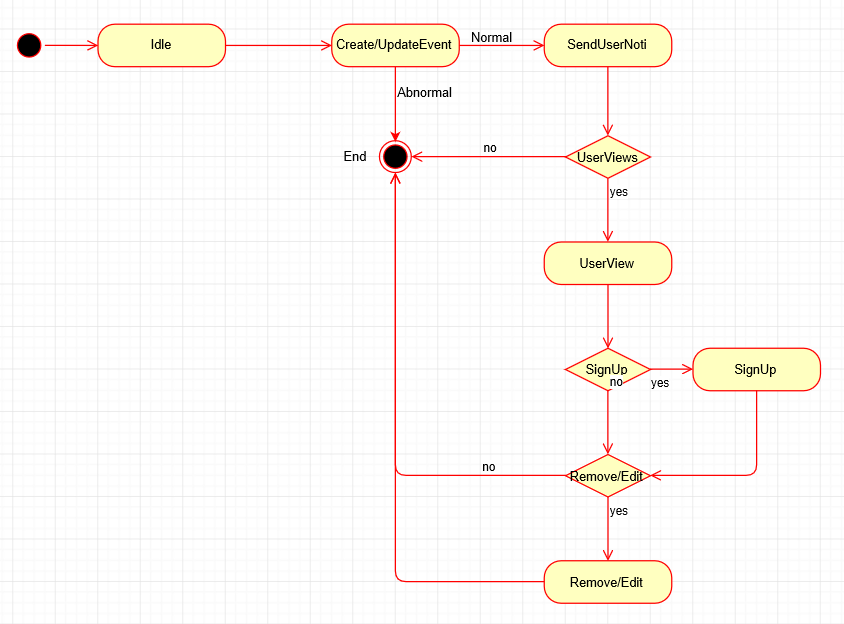
\includegraphics[width=\textwidth]{event/StateDiagramTask2.PNG}
		\caption{Events State Diagram}
\end{figure}




\subsubsection{Use Case Diagram}
Use case diagram which shows the functions of the subsystem as well as relationships of external entities or actors. This refined version also includes a detailed flow of use cases.
\begin{figure}[H]
		\centering
		\includegraphics[width=0.7\textwidth]{event/UserCaseTask2.PNG}
		\caption{Events core functionality }
\end{figure}


